\documentclass[tikz,border=10pt]{standalone}
\usepackage{amsmath}
\usepackage{amssymb}

\usetikzlibrary{arrows.meta, positioning, calc}

\begin{document}

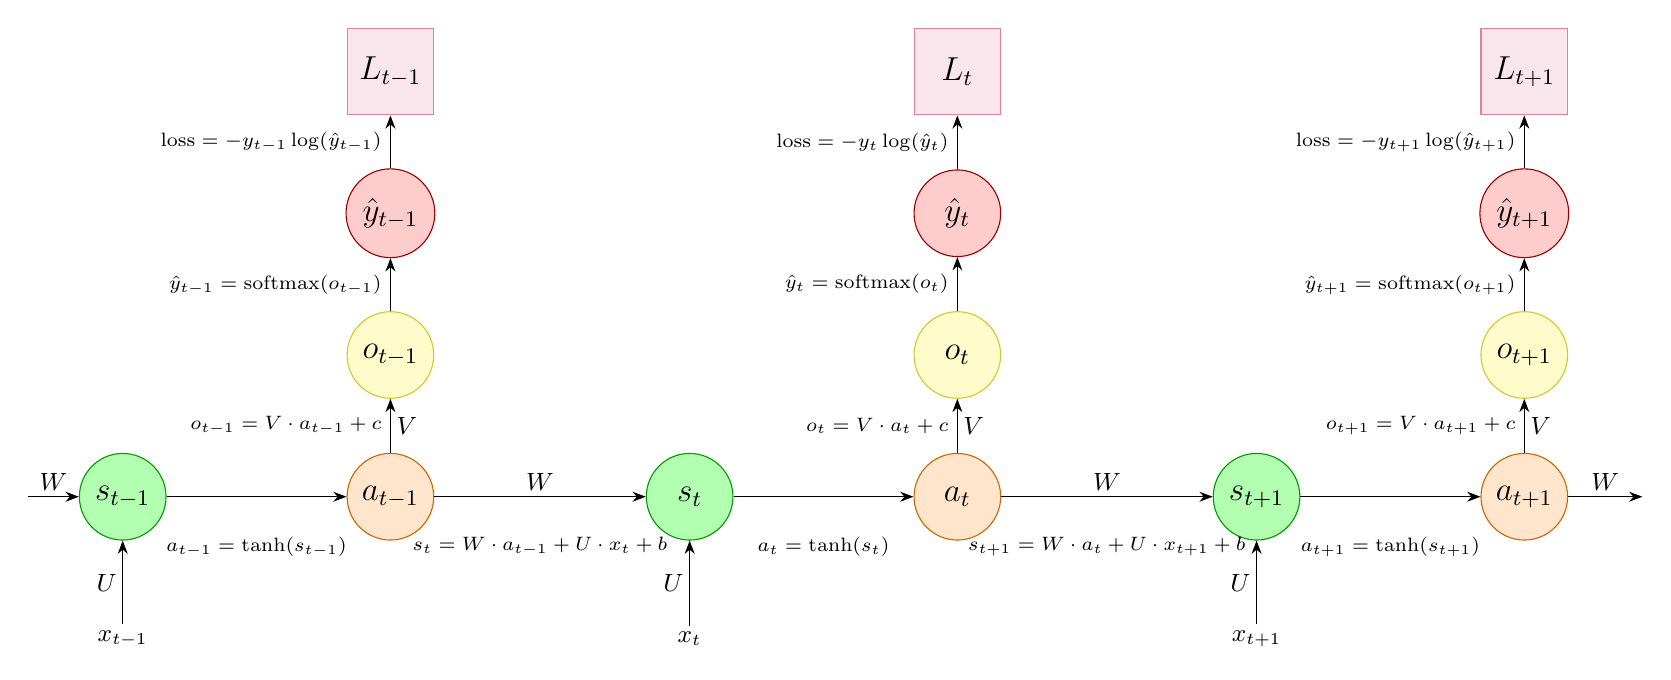
\begin{tikzpicture}[
    >=Stealth,
    % Define the matching styles from the diagram
    s_node/.style={circle, draw=green!60!black, fill=green!30, minimum size=1.1cm, font=\large},
    a_node/.style={circle, draw=orange!80!black, fill=orange!20, minimum size=1.1cm, font=\large},
    o_node/.style={circle, draw=yellow!80!black, fill=yellow!20, minimum size=1.1cm, font=\large},
    y_node/.style={circle, draw=red!60!black, fill=red!20, minimum size=1.1cm, font=\large},
    loss_node/.style={rectangle, draw=purple!50, fill=purple!10, minimum size=1.1cm, font=\large},
    lbl/.style={font=\small, inner sep=2pt},
    math_lbl/.style={font=\scriptsize, inner sep=3pt} % Added a tiny bit of extra padding
]

    % Global horizontal spacing control between time steps
    \newcommand{\spacing}{7.2} 

    % Loop to generate the 3 time steps: t-1 (i=0), t (i=1), t+1 (i=2)
    \foreach \i/\sub in {0/{t-1}, 1/{t}, 2/{t+1}} {
        \coordinate (origin) at (\i*\spacing, 0);
        
        % --- Bottom Row Nodes ---
        \node[s_node] (s_\i) at ($(origin) + (0,0)$) {$s_{\sub}$};
        \node[a_node] (a_\i) at ($(s_\i) + (3.4, 0)$) {$a_{\sub}$}; 
        \node[lbl] (x_\i) at ($(s_\i) + (0, -1.8)$) {$x_{\sub}$};
        
        % --- Vertical Columns ---
        \node[o_node] (o_\i) at ($(a_\i) + (0, 1.8)$) {$o_{\sub}$};
        \node[y_node] (y_\i) at ($(o_\i) + (0, 1.8)$) {$\hat{y}_{\sub}$};
        \node[loss_node] (L_\i) at ($(y_\i) + (0, 1.8)$) {$L_{\sub}$};
        
        % --- Inside-Step Arrows ---
        \draw[->] (x_\i) -- node[left, lbl] {$U$} (s_\i);
        
        % MOVED BELOW: Internal activation function equation
        \draw[->] (s_\i) -- node[below, math_lbl,yshift=-4mm] {$a_{\sub} = \tanh(s_{\sub})$} (a_\i);
        
        \draw[->] (a_\i) -- node[right, lbl] {$V$} node[left, math_lbl] {$o_{\sub} = V \cdot a_{\sub} + c$} (o_\i);
        \draw[->] (o_\i) -- node[left, math_lbl] {$\hat{y}_{\sub} = \text{softmax}(o_{\sub})$} (y_\i);
        \draw[->] (y_\i) -- node[left, math_lbl] {$\text{loss} = -y_{\sub}\log(\hat{y}_{\sub})$} (L_\i);
    }

    % --- Cross-Step Connections (Horizontal Flow) ---
    
    % Edge into t-1
    \draw[->] ($(s_0) - (1.2, 0)$) -- node[above, lbl] {$W$} (s_0);
    
    % Connection from t-1 to t (Formula below, W weight above)
    \draw[->] (a_0) -- node[below, math_lbl,yshift=-4mm] {$s_t = W \cdot a_{t-1} + U \cdot x_t + b$} node[above, lbl] {$W$} (s_1);
    
    % Connection from t to t+1 (Formula below, W weight above)
    \draw[->] (a_1) -- node[below, math_lbl,yshift=-4mm] {$s_{t+1} = W \cdot a_{t} + U \cdot x_{t+1} + b$} node[above, lbl] {$W$} (s_2);
    
    % Edge exiting t+1
    \draw[->] (a_2) -- node[above, lbl] {$W$} ($(a_2) + (1.5, 0)$);

\end{tikzpicture}
\end{document}